\documentclass[__main__.tex]{subfiles}

\begin{document}

\paragraph{Э-02}
Рассмотрите электромагнитные волны в пространстве, свободном от зарядов и токов. Покажите, что вектора $\vec{k}$ (волновой вектор), $\vec{E}$, $\vec{B}$ образуют правую тройку в некоторой инерциальной системе отсчёта. Объясните, почему в любой другой инерциальной системе отсчёта этот факт, будучи сформулированным для преобразованных векторов, будет также иметь место.\\

Вектор $k = \frac{\omega}{V} n$, где $n$ - единичный вектор распространения волны, $V$ - скорость распространения волны, называется \textbf{волновым вектором}.

Процесс распространения электромагнитного поля в пространстве называется электромагнитной волной. 

\begin{enumerate}
\item
Электромагнитная волна поперечна, колебания векторов $E$ и $B$ проходят перпендикулярно направлению распространения волны (см. Рис. 80);
\item
Электрическое и магнитное поля в бегущей волне изменяются в одной фазе;
\item
Вектора $E$,$B$ и $V$ (а вместе с ним и $k$) в бегущей электромагнитной волне образуют так называемую правую тройку векторов.
\end{enumerate}

\begin{figure}[h]
\begin{minipage}{.45\linewidth}
    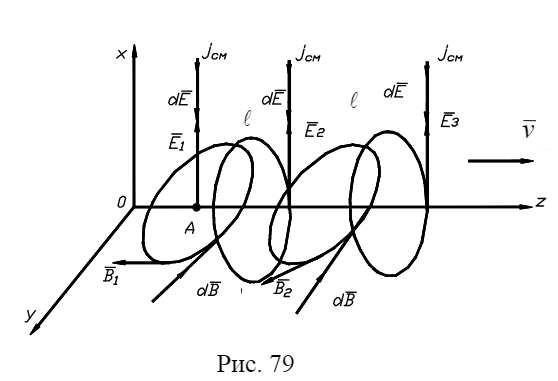
\includegraphics[width=1\linewidth]{e02_1}
\end{minipage}
\hfill
\begin{minipage}{.45\linewidth}
    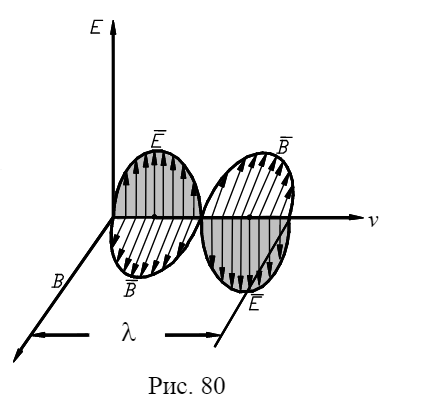
\includegraphics[width=1\linewidth]{e02_2}
\end{minipage}
\end{figure}

\end{document}
